%!TEX root = ../FundationsDataScience.tex

\chapter{Machine Learning}

% probabilistic variables
\newcommand{\xp}{\mathrm{\bf x}}
\newcommand{\yp}{\mathrm{\bf y}}

% Refs \cite{rosasco2017notes,friedman2001elements,murphy2012machine}

This chapter gives a rapid overview of the main concepts in machine learning. The goal is not to be exhaustive, but to highlight representative problem to insist on the distinction between unsupervised (vizualization and clustering) and supervised (regression and classification) problems. We also shed light on the tight connexions between machine learning and inverse problems. 


%%%%%%%%%%%%%%%%%%%%%%%%%%%%%%%%%%%%%%%%%%%%%%%%%%
%%%%%%%%%%%%%%%%%%%%%%%%%%%%%%%%%%%%%%%%%%%%%%%%%%
%%%%%%%%%%%%%%%%%%%%%%%%%%%%%%%%%%%%%%%%%%%%%%%%%%
\section{Unsupervised Learning}

In unsupervised learning, one observed $n$ points $(x_i)_{i=1}^n$. For simplicity, we assume the data are point in Euclidean space $x_i \in \RR^p$ ($p$ is the so-called number of features). These points are conveniently stored as the rows of a matrix $X \in \RR^{n \times d}$.
%
The problem is now to infer some properties for this points, typically for vizualization or unsupervised classication (often called clustering). 


%%%%%%%%%%%%%%%%%%%%%%%%%%%%%%%%%%%%%%%%%%%%%%%%%%
\subsection{Dimensionality Reduction and PCA}

Dimensionality reduction is useful for vizualization. It can also be understood as the problem of feature extraction (determining which are the relevant parameters), and this can be later used for doing other tasks more efficiently (faster and/or with better performances). 


In order to display in 2-D or 3-D the data, dimensionality reduction is needed.
The simplest method is the Principal Component Analysis (PCA),  which perform an orthogonal linear projection on the principal axis (eigenvector) of the covariance matrix.

The empirical mean is defined as 
\eq{
    \hat m \eqdef \frac{1}{n} \sum_{i=1}^n x_i \in \RR^p
} 
and  covariance
\eql{\label{eq-emp-cov}
 	\hat C \eqdef \frac{1}{n} \sum_{i=1}^n (x_i-m) (x_i-m)^\top \in \RR^{p \times p}. 
}
Denoting $\tilde X = X - 1_p \hat m^\top $, one has $\hat C=\tilde X^\top
\tilde X$. 

Note that if points $(x_i)_i$ are actually i.i.d. variable, and denoting $x$ one of these random variable, one has using the law of large number, the almost surely convergence as $n \rightarrow +\infty$
\eql{\label{eq-cov-approx}
	\hat m \rightarrow m \eqdef \EE(x)
	\qandq
	\hat C \rightarrow C \eqdef \EE((x-m)(x-m)^\top).
}
Denoting $\mu$ the distribution (Radon measure) on $\RR^p$ of $x$, one can alternatively write
\eq{
	m = \int_{\RR^p} x \d\mu(x)
	\qandq
	C = \int_{\RR^p} (x-m)(x-m)^\top \d\mu(x).	
}


\begin{figure}
\centering
\begin{tabular}{@{}c@{}c@{}}
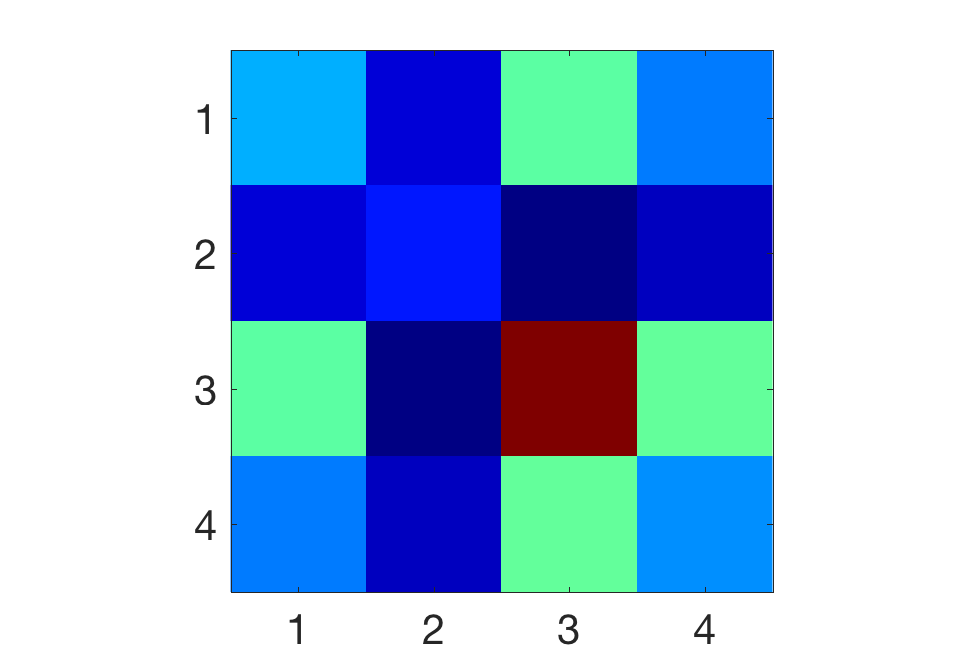
\includegraphics[width=.25\linewidth]{ml/pca-nn/cov}&
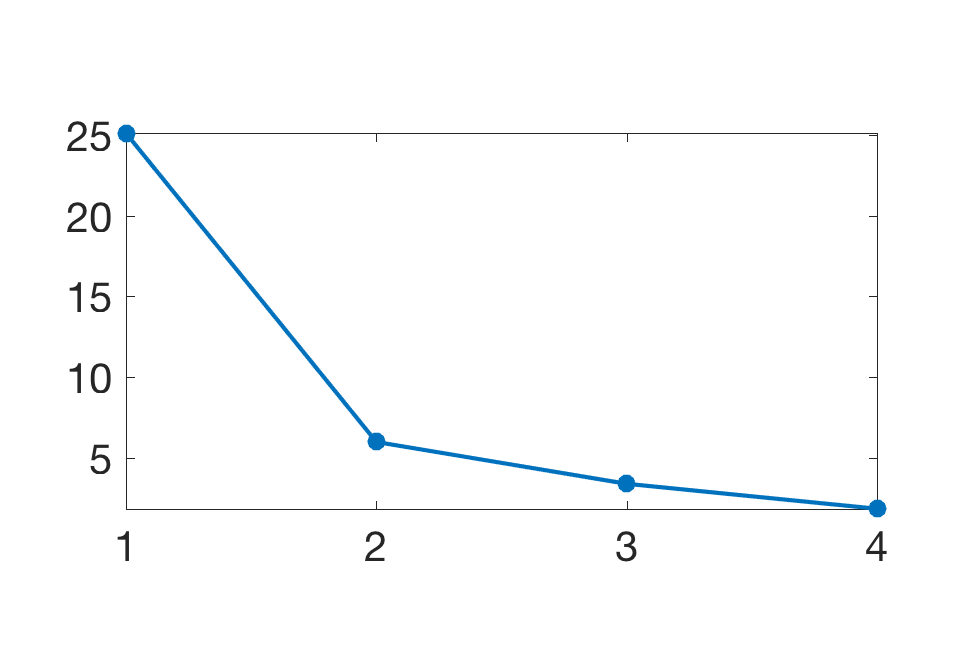
\includegraphics[width=.4\linewidth]{ml/pca-nn/svd}\\
$C$ & SVD of $C$
\end{tabular}
\caption{\label{fig-cov}
Empirical covariance of the data and its associated singular values. 
}
\end{figure}

The PCA ortho-basis, already introduced in Section~\ref{prop-svd}, corresponds to the right singular vector of the centred data matrix using the (reduce) SVD decomposition
\eq{
 	\tilde X = U \diag(\si) V  
}
where $U \in \RR^{n \times r}$ and $V \in \RR^{p \times r}$, and where $r=\rank(\tilde X) \leq \min(n,p)$. In usual settings, $n \gg p$, and one assume having enough samples so that the approximation~\eqref{eq-cov-approx}. 
%
We denote $V=(v_k)_{k=1}^r$ the orthogonal columns $v_k \in \RR^p$. The intuition is that they are the main axis of ``gravity'' of the cloud $X$.
%
We assume the singular are order, $\si_1 \geq \ldots \geq \si_r$, so that the first singular values capture most of the variance. 


Figure~\ref{fig-cov} displays an example of covariance and its associated spectrum $\si$. The points $(x_i)_i$ corresponds to the celebrated
IRIS dataset\footnote{\url{https://en.wikipedia.org/wiki/Iris_flower_data_set}} of Fisher.  This dataset consists of 50 samples from each of three species of Iris (Iris setosa, Iris virginica and Iris versicolor). Four $d=4$ were measured from each sample: the length and the width of the sepals and petals, in centimetres. 


The PCA dimensionality reduction embedding $x_i \in \RR^p \mapsto z_i \in \RR^d$ in dimension $d \leq p$ is obtained by projecting on the first $d$ singular vector
\eq{
	z_i \eqdef ( \dotp{x_i-m}{v_k} )_{k=1}^d \in \RR^d. 
}
From these low-dimensional embedding, one can reconstruct back an approximation as
\eq{
	\tilde x_i \eqdef m+\sum_k z_{i,k} v_k \in \RR^p.
}
One has that $\tilde x_i = \Proj_{\tilde T}(x_i)$ where $\tilde T \eqdef m + \Span_{k=1}^d(v_k)$ is an affine space.
%
The following proposition shows that PCA is optimal in term of $\ell^2$ distance if one consider only affine spaces.

\begin{prop}
	One has
	\eq{
		(\tilde x,\tilde T) \in \uargmin{ (\bar x,\bar T) } \enscond{ \sum_i \norm{x_i - \bar x_i }^2 }{ \foralls i, \bar x_i \in \bar T }
	}
	where $\bar T$ is constrained to be a $d$-dimensional affine space. 
\end{prop}


Figure~\ref{fig-pca} shows an example of PCA for 2-D and 3-D vizualization.


\begin{figure}
\centering
\begin{tabular}{@{}c@{\hspace{5mm}}c@{}}
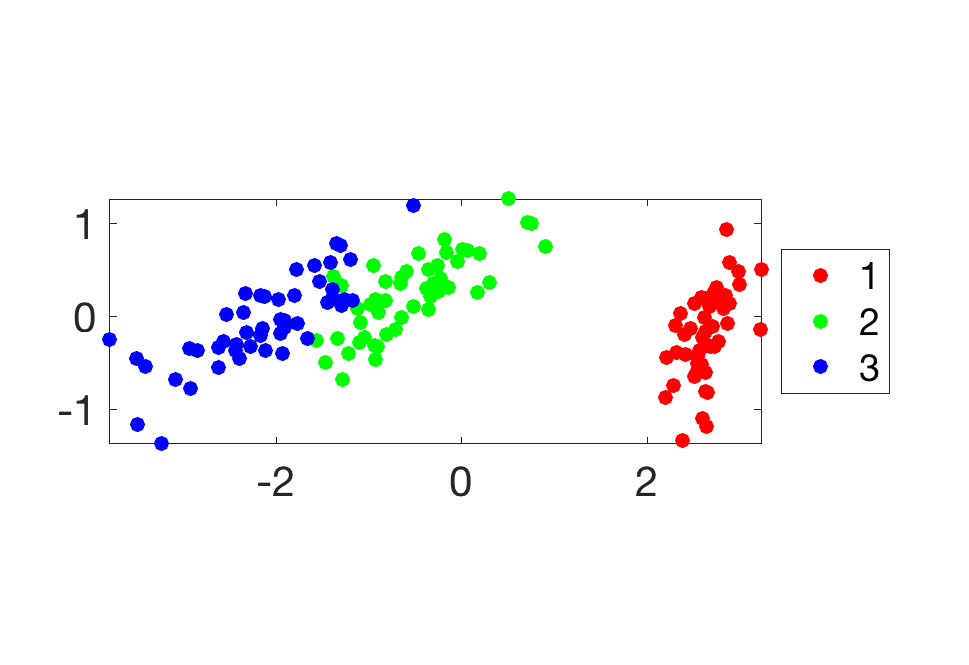
\includegraphics[width=.4\linewidth]{ml/pca-nn/points-2d}&
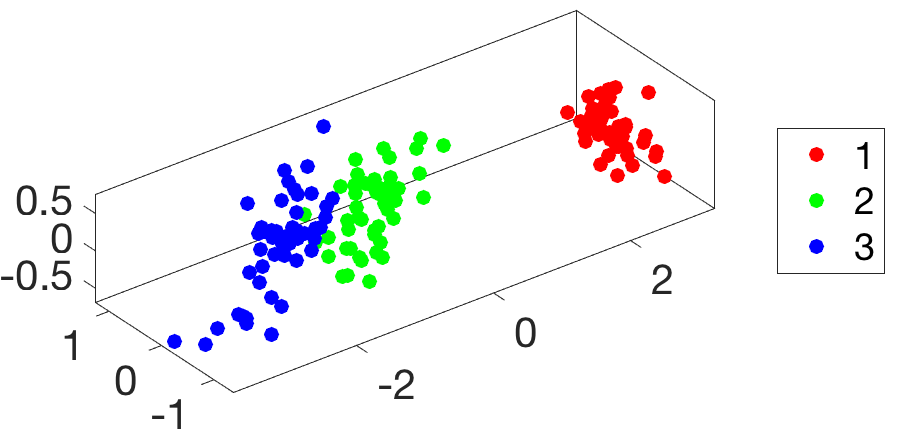
\includegraphics[width=.4\linewidth]{ml/pca-nn/points-3d}
\end{tabular}
\caption{\label{fig-pca}
2-D and 3-D PCA vizualization of the input clouds. 
}
\end{figure}



%%%%%%%%%%%%%%%%%%%%%%%%%%%%%%%%%%%%%%%%%%%%%%%%%%%%%%%%%%%%%%%%%%
\subsection{Clustering and $k$-means}

A typical unsupervised learning task is to infer a class label $y_i \in \{1,\ldots,k\}$ for each input points $x_i$, and this is often called a clustering problems (since the set of points associated to a given label can be thought as a cluster).

%%%%
\paragraph{$k$-means}

A way to infer these label is by assuming that the cluster are compact, and optimizing a compactness criterion. Assuming for simplicity that the data are in Euclidean space (which can be relaxed to an arbitrary metric space, although the computation become more complicated), the $k$-means approach minimizes the distance between the points and their class centroids $c=(c_\ell)_{\ell=1}^k$, where each $c_\ell \in \RR^p$. The corresponding variational problem becomes
\eq{
	\umin{ (y,c) } \Ee( y, c ) \eqdef \sum_{\ell=1}^k \sum_{ i : y_i=\ell } \norm{x_i-c_\ell}^2. 
}

The $k$-means algorithm can be seen as a block coordinate relaxation, which alternatively update the class label and the centroids.
%
The centroids $c$ are first initialized (more on this later), for instance, using a well-spread set of points from the samples.  
% 
For a given set $c$ of centroids, minimizing $y \mapsto \Ee(y,c)$ is obtained in closed form by assigning as class label the index of the closest centroids
\eql{\label{eq-kmeans-1}
	\foralls i \in \{1,\ldots,n\}, \quad y_i \leftarrow \uargmin{1 \leq \ell \leq k} \norm{x_i-c_\ell}.
}
For a given set $y$ of centroids, minimizing $c \mapsto \Ee(y,c)$ is obtained in closed form by computing the barycenter of each class
\eql{\label{eq-kmeans-2}
	\foralls \ell \in \{1,\ldots,k\}, \quad c_\ell \leftarrow \frac{
		\sum_{i : y_i=\ell} x_i
	}{
		|\enscond{i}{y_i=\ell}|
	}
}
If during the iterates, one of the cluster associated to some $c_\ell$ become empty, then one can either decide to destroy it and replace $k$ by $k-1$, or try to ``teleport'' the center $c_\ell$ to another location (this might increase the objective function $\Ee$ however). 

Since the energy $\Ee$ is decaying during each of these two steps, it is converging to some limit value. Since there is a finite number of possible labels assignments, it is actually constant after a finite number of iterations, and the algorithm stops. 

Of course, since the energy is non-convex, little can be said about the property of the clusters output by $k$-means.
%
To try to reach lower energy level, it is possible to ``teleport'' during the iterations centroids $c_\ell$ associated to cluster with high energy to location within cluster with lower energy (because optimal solutions should somehow balance the energy).  

Figure~\ref{fig-kmeans} shows an example of $k$-means iterations on the Iris dataset.

\begin{figure}
\centering
\begin{tabular}{@{}c@{\hspace{10mm}}c@{}}
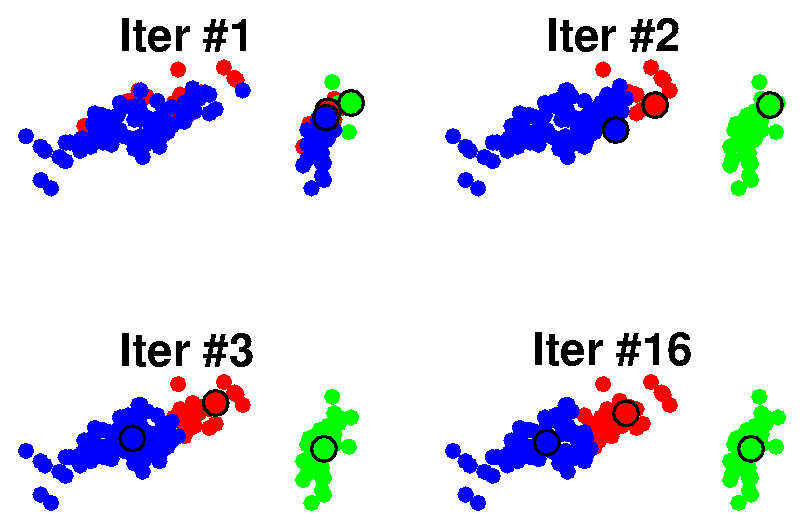
\includegraphics[width=.4\linewidth]{ml/pca-nn/kmeans-iter}&
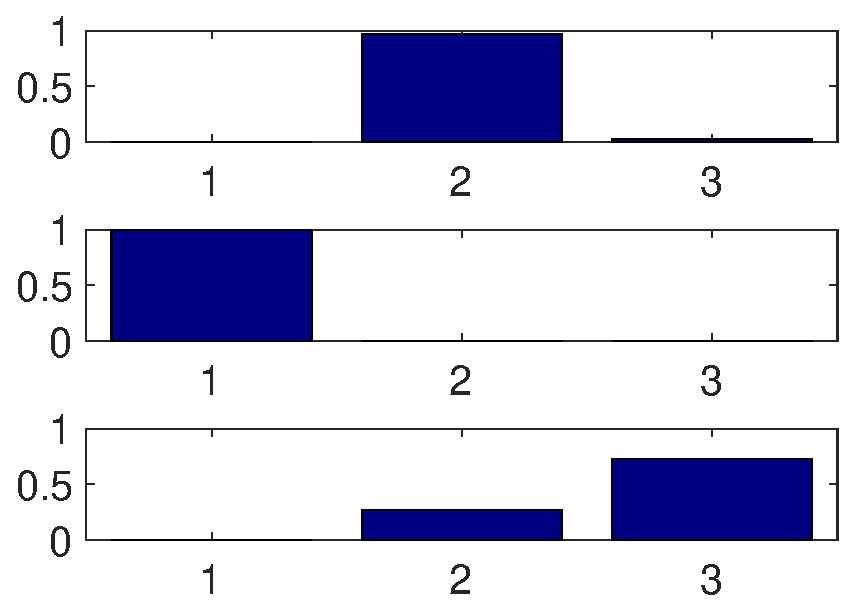
\includegraphics[width=.35\linewidth]{ml/pca-nn/kmeans-classif-scores}
\end{tabular}
\caption{\label{fig-kmeans}
Left: iteration of $k$-means algorithm. Right: histogram of points belonging to each class. 
}
\end{figure}


%%%%
\paragraph{$k$-means++}

The crucial point to obtain good results when using $k$-means is to have an efficient initialization. In practice, the best results are obtained by seeding them as far as possible from one another (a greedy strategy works great in practice). 

Quite surprisingly, there exists a randomized seeding strategy which can be shown to be closed to optimal, even without running the $k$-means iterations (although in practice it is still required to obtain descent results). The corresponding $k$-means++ initialization is obtained by selecting $c_1$ uniformly at random among the $x_{i}$, and then assuming $c_\ell$ has been seeded, drawing $c_{\ell+1}$ according to the probability $\pi^{(\ell)}$ on $\{1,\ldots,n\}$ proportional to the square of the distance to the previously seeded points
\eq{
	\foralls i \in \{1,\ldots,n\}, \quad 
	\pi^{(\ell)}_i \eqdef \frac{ d_i^2 }{ \sum_{j=1}^n d_j^{2} }
	\qwhereq
	d_j \eqdef \min_{1 \leq r \leq \ell-1} \norm{x_i-c_r}^{2}
}

The following results, due to David Arthur and Sergei Vassilvitskii shows that this seeding is optimal up to log factor on the energy. Note that finding a global optimum is known to be NP-hard.

\begin{thm}
	For the centroids $c^\star$ defined by the $k$-means++ strategy, denoting $y^\star$ the associated nearest neighbor labels defined as in~\eqref{eq-kmeans-1}, one has
	\eq{
		\EE(\Ee(y^\star,c^\star)) \leq 8 (2+\log(k)) \umin{(y,c)} \Ee(y,v). 
	}
	where the expectation is on the random draws of performed by the algorithm.
\end{thm}




%%%%
\paragraph{Lloyd algorithm and continuous densities.}

The $k$-means iterations are also called ``Lloyd'' algorithm, which also find popular application to optimal vector quantization for compression. It can also be used in the ``continuous'' setting where the empirical samples $(x_i)_i$ are replaced by an arbitrary measure over $\RR^P$. 
%
The energy to minimize becomes
\eq{
	\umin{ (\Vv,c) } \sum_{\ell=1}^k \int_{\Vv_\ell} \norm{x-c_\ell}^2 \d \mu(x)
}
where $(\Vv_\ell)_\ell$ is a partition of the domain. 
%
Step~\eqref{eq-kmeans-1} is replaced by the computation of a Voronoi cell
\eq{
	\foralls \ell \in \{1,\ldots,k\}, \quad 
	\Vv_\ell \eqdef \enscond{x}{ \foralls \ell' \neq \ell, \norm{x-c_\ell} \leq \norm{x-c_{\ell'}} }.
}
These Voronoi cells are polyhedra delimited by segments of mediatrix between centroids, and this Voronoi segmentation can be computed efficiently using tools from algorithmic geometry in low dimension. 
%
Step~\eqref{eq-kmeans-2} are then replaced by
\eq{
	\foralls \ell \in \{1,\ldots,k\}, \quad c_\ell \leftarrow \frac{
		\int_{\Cc_\ell} x \d\mu(x)
	}{
		\int_{\Cc_\ell} \d\mu(x)
	}.
}
In the case of $\mu$ being uniform distribution, optimal solution corresponds to the hexagonal lattice.
%
Figure~\ref{fig-lloyd} displays two examples of Lloyd iterations on 2-D densities on a square domain.

\begin{figure}
\centering
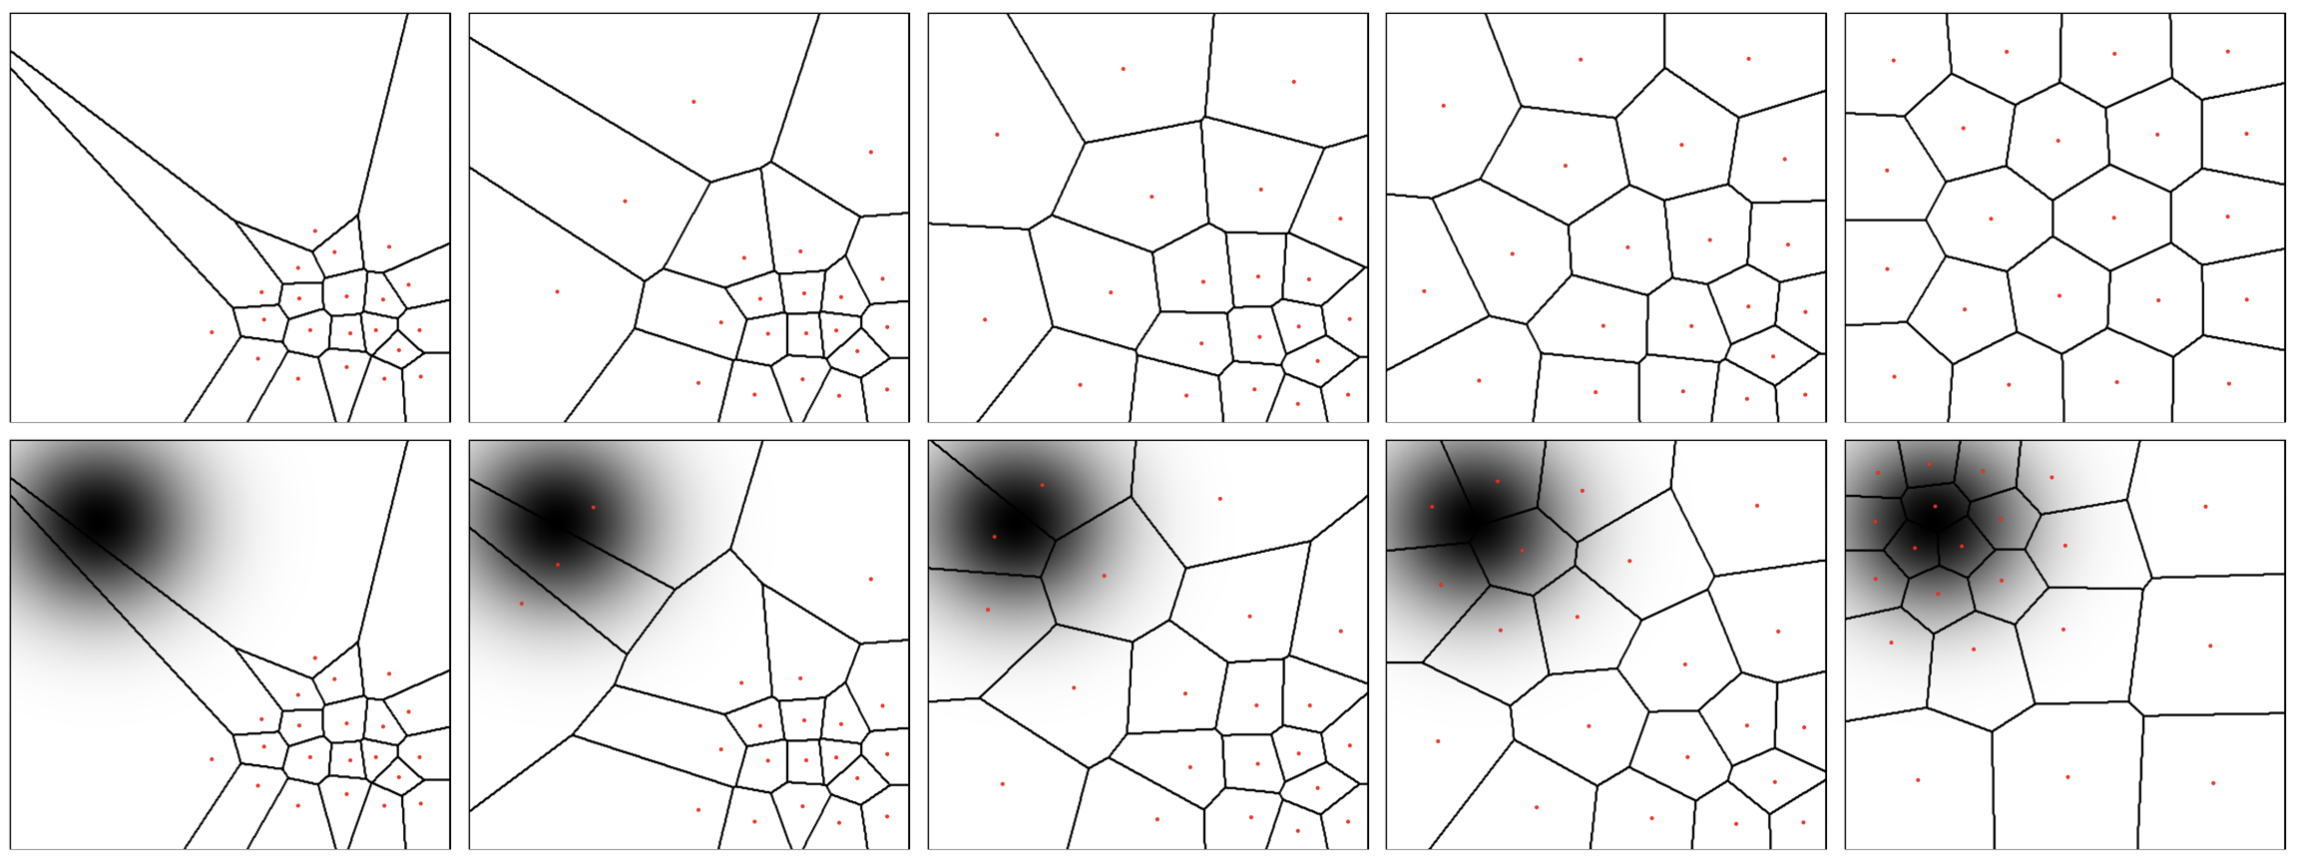
\includegraphics[width=\linewidth]{ml/pca-nn/lloyd}
\caption{\label{fig-lloyd}
Iteration of $k$-means algorithm (Lloyd algorithm) on continuous densities $\mu$. Top: uniform. Bottom: non-uniform (the densities of $\mu$ with respect to the Lebesgue measure is displayed as a grayscale image in the background).
}
\end{figure}



%%%%%%%%%%%%%%%%%%%%%%%%%%%%%%%%%%%%%%%%%%%%%%%%%%
%%%%%%%%%%%%%%%%%%%%%%%%%%%%%%%%%%%%%%%%%%%%%%%%%%
%%%%%%%%%%%%%%%%%%%%%%%%%%%%%%%%%%%%%%%%%%%%%%%%%%
\subsection{Supervised Learning: Regression}

\wrapf{ml/proba-model}{Probabilistic modelling.}
In supervised learning, one has access to training data, consisting in pairs $(x_i,y_i) \in \Xx \times \Yy$. Here $\Xx=\RR^p$ for simplicity. The goal is to infer some relationship, typically of the form $y_i \approx f(x_i)$ for some deterministic function $f : \Xx \rightarrow \Yy$, in order, when some un-observed data $x$ without associated value in $\Yy$ is given, one can ``predict'' the value using $y = f(x)$. 

If the set $\Yy$ is discrete and finite, then this problem is called a supervised classification problem, and this is specifically studied in Section~\ref{sec-classif}. The simplest example being the binary classification case, $\Yy=\{0,1\}$, for instance in medical diagnosis, $y_i=0$ indicate a healthy subject, why $y_i=0$ a pathological one.
%
If $\Yy$ is continuous (the typical example being $\Yy=\RR$), then this problem is called a regression problem. 

%%%%%%%%%%%%%%%%%%%%%%%%%%%%%%%%%%%%%%%%%%%%%%%%%%
\subsection{Empirical Risk Minimization}

In order to make the problem tractable computationally, and also in order to obtain efficient prediction score, it is important to restrict the fit to the data $y_i \approx f(x_i)$ using a restricted class of functions. Intuitively, in order to avoid overfitting, the ``size'' of this class of function should grows with the number $n$ of samples. 

%%%
\paragraph{Empirical risk.}

Denoting $\Ff_n$ some class of function, the most usual way to do the learning is to perform an empirical risk minimization (ERM)
\eql{\label{eq-erm-1}
	\hat f \in \uargmin{f \in \Ff_n} \frac{1}{n} \sum_{i=1}^n \Ll(f(x_i),y_i).
}
Here $\Ll : \Yy^2 \rightarrow \RR^+$ is the so-called loss function, and it should typically satisfies $\Ll(y,y')=0$ if and only if $y=y'$. The specifics of $\Ll$ depends on the applications (in particular, one should use different loss for classification and regression tasks). 
%
To highlight the dependency of $\hat f$ on $n$, we occasionally write $\hat f_n$. 


%%%
\paragraph{Prediction risk and prediction consistency.}

When doing a mathematically analysis, one usually assume that $(x_i,y_i)$ are drawn from a distribution $\pi$ on $\Xx \times \Yy$, and the large $n$ limit defines the ideal estimator
\eql{\label{eq-consistency-estim}
	\bar f \in \uargmin{f \in \Ff_n} \int_{\Xx \times \Yy} \Ll(f(x),y) \d\pi(x,y) = \EE_{(\xp,\yp) \sim \pi}(\Ll(f(\xp),\yp).
}
Intuitively, one should have $\hat f_n \rightarrow \bar f$ as $n \rightarrow +\infty$, which can be captured in expectation of the prediction error over the samples $(x_i,y_i)_i$, i.e.
\eq{
	E_n \eqdef \EE( \tilde\Ll(\hat f_n(\xp),f(\xp)) ) \longrightarrow 0.
}
One should be careful that here the expectation is over both $\xp$ (distributed according to the marginal $\pi_\Xx$ of $\pi$ on $\Xx$), and also the $n$ i.i.d. pairs $(x_i,y_i) \sim \pi$ used to define $\hat f_n$ (so a better notation should rather be $(\xp_i,\yp_i)_i$.
%
Here $\bar\Ll$ is some loss function on $\Yy$ (one can use $\bar\Ll=\Ll$ for instance).
One can also study convergence in probability, i.e. 
\eq{
	\foralls \epsilon>0, \quad
	E_{\epsilon,n} \eqdef \PP( \tilde\Ll(\hat f_n(\xp),f(\xp)) > \epsilon ) \rightarrow 0.
}
If this holds, then one says that the estimation method is consistent (in expectation or in probability). 
%
The question is then to derive convergence rates, i.e. to upper bound $E_n$ or $E_{\epsilon,n}$ by some explicitly decay rate. 

Note that when $\tilde\Ll(y,y')=|y-y'|^r$, then convergence in expectation is stronger (implies) than convergence in probability since using Markov's inequality
\eq{
	E_{\epsilon,n} = \PP( |\hat f_n(\xp)-f(\xp)|^r \geq \epsilon )  \leq \frac{1}{\epsilon} \EE( |\hat f_n(\xp)-f(\xp)|^r ) = \frac{E_n}{\epsilon}.
}

%%%
\paragraph{Parametric approach and regularization.}

Instead of directly defining the class $\Ff_n$ and using it as a constraint, it is possible to rather use a penalization using some prior to favor ``simple'' or ``regular'' functions. 
%
This can also be enforced using parametric models $y \approx f(x,\be)$ where $\be \in \Bb$ parametrizes the function $f(\cdot,\th) : \Xx \rightarrow \Yy$. The empirical risk minimization procedure~\eqref{eq-erm-1} now becomes 
\eql{\label{eq-erm-1}
	\hat \be \in \uargmin{\be \in \Bb} \frac{1}{n} \sum_{i=1}^n \Ll(f(x_i,\be),y_i) + \la_n J(\be).
}
where $J$ is some regularization function, for instance $J=\norm{\cdot}_2^2$ or $J=\norm{\cdot}_1$. Here $\la_n>0$ is a regularization parameter, and it should tend to $0$ when $n \rightarrow 0$. 

Then one similarly defines the ideal parameter $\bar \be$ as in~\eqref{eq-consistency-estim} so that the limiting estimator as $n \rightarrow +\infty$ is of the form $\bar f = f(\cdot,\bar \be)$. 

In this parametric approach, one could be interested in also studying how close $\hat \th$ is close to $\bar \th$. This can be measure by controlling how fast some estimation error $\norm{\hat\th-\bar\th}$ (for some norm $\norm{\cdot}$) goes to zero. Note however that in most cases, controlling the estimation error is much more difficult than doing the same for the prediction error. Doing a good parameter estimation implies doing a good prediction, but the converse is not true. 


%%%
\paragraph{Testing set.}

In practice, $E_n$ or $E_{\epsilon,n}$ are ideal quantity which cannot be accessed. One thus rather ressort to a second set of data $(\bar x_j,\bar y_j)_{j=1}^{\bar n}$, called ``testing set''. From a modelling perspective, this set should also be distributed i.i.d. according to $\pi$. The validation (or testing) risk is then
\eql{\label{eq-valid-risk}
	R_{\bar n} = \frac{1}{\bar n} \sum_{j=1}^{\bar n} \Ll(\hat f(\bar x_j),\bar y_j).
}
Minimizing $R_{\bar n}$ to setup to some meta-parameter of the method (for instance the regularization parameter $\la_n$) is called ``cross validation'' in the litterature.


%%%%%%%%%%%%%%%%%%%%%%%%%%%%%%%%%%%%%%%%%%%%%%%%%%
\subsection{Linear Regression}
\label{sec-linear-models}

We now specialized the empirical risk minimization approach to regression problem, and even more specifically, we consider $\Yy=\RR$ and use a quadratic loss $\Ll(y,y')=\frac{1}{2}|y-y'|^2$.

%%%
\paragraph{Least square and conditional expectation.}

If one do not put any constraint on $f$ (beside being measurable), then the optimal limit estimator $\bar f(x)$~\eqref{eq-consistency-estim} is simply averaging the values $y$ sharing the same , which is the so-called conditional expectation. 
%
Assuming for simplicity that $\pi$ has some density $\frac{\d \pi}{\d x \d y}$ with respect to a tensor product measure $\d x \d y$ (for instance the Lebegues mesure), one has
\eq{
	\foralls x \in \Xx, \quad
	\bar f(x) = \EE( \yp | \xp=x) = 
	\frac{ 
		\int_{\Yy} y \frac{\d \pi}{\d x \d y}(x,y) \d y 
	}{ 
		\int_{\Yy} \frac{\d \pi}{\d x \d y}(x,y) \d y
	 }
}
where $(\xp,\yp)$ are distributed according to $\pi$.



\begin{figure}
\centering
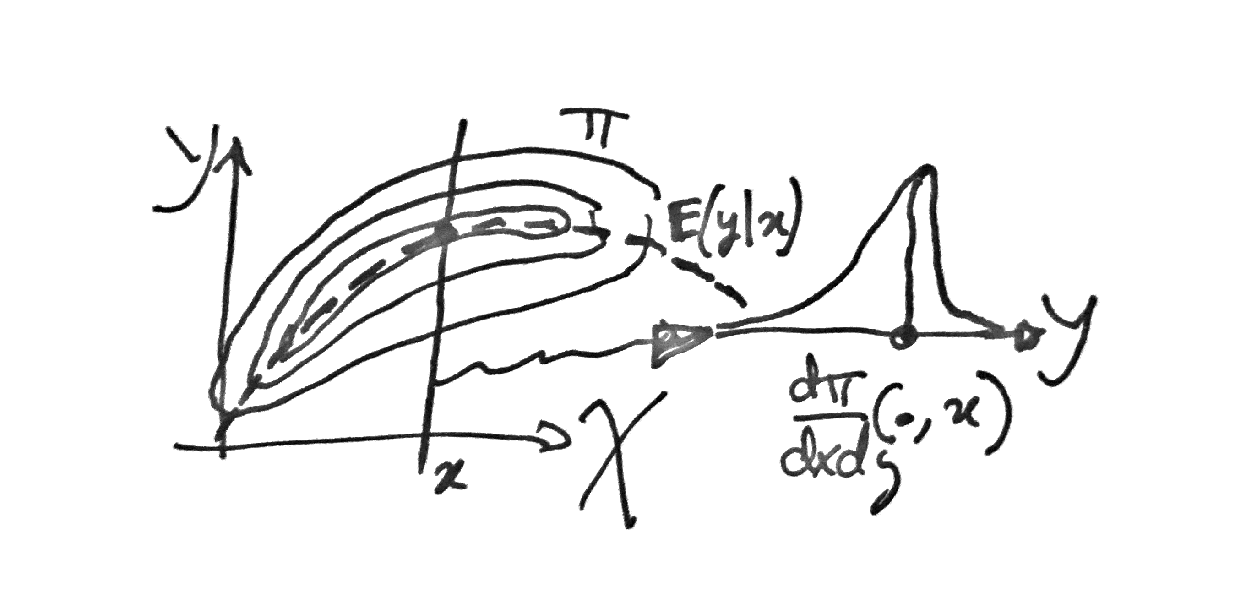
\includegraphics[width=.5\linewidth]{ml/cond-expect}
\caption{\label{fig-bound-regul}
Conditional expectation.
}
\end{figure}

In the simple case where $\Xx$ and $\Yy$ are discrete, denoting $\pi_{x,y}$ the probability of $(\xp=x,\yp=y)$, one has
\eq{
	\foralls x \in \Xx, \quad
	\bar f(x) = \frac{ \sum_{y}  y \pi_{x,y} }{ \sum_{y} \pi_{x,y} }
}
and it unspecified if the marginal of $\pi$ along $\Xx$ vanishes at $x$. 

The main issue is that the estimator $\hat f$ performs very poorly on finite sample, and $f(x)$ is actually undefined if there is no sample $x_i$ equal to $x$. This is due to the fact that the class of functions is too large, and one should impose some regularity or simplicity on the set of admissible $f$.


%%%
\paragraph{Penalized linear models.}

A very simple class of model is obtained by imposing that $f$ is linear, and set $f(x,\be)=\dotp{x}{\be}$, for parameter $\be \in \RR^p$. Note that one can also treat this way affine function by remarking that $\dotp{x}{\be}+\be_0=\dotp{(x,1)}{(\be,\be_0)}$ and replacing $x$ by $(x,1)$. 

Under the square loss, the regularized ERM~\eqref{eq-erm-1} is conveniently rewritten as 
\eql{\label{eq-erm-lin}
	\hat \be \in \uargmin{\be \in \Bb} \frac{1}{2} \dotp{\hat C \be}{\be} - \dotp{\hat u}{\be} + \la_n J(\be)
}
where we introduced the empirical correlation (already introduced in~\eqref{eq-emp-cov}) and observations
\eq{
	\hat C \eqdef \frac{1}{n} X^* X = \frac{1}{n} \sum_{i=1}^n x_i x_i^*
	\qandq
	\hat u \eqdef \frac{1}{n} \sum_{i=1}^n y_i x_i = \frac{1}{n} X^* y \in \RR^p.
}
As $n \rightarrow 0$, under weak condition on $\pi$, one has with the law of large number the almost sure convergence
\eql{\label{eq-empirical-conver}
	\hat C \rightarrow C \eqdef \EE(\xp^* \xp)
	\qandq
	\hat u \rightarrow C \eqdef \EE(\yp \xp).
}
When considering $\la_n \rightarrow 0$, in some case, one can shows that in the limit $n \rightarrow +\infty$ (under some additional condition on the decay), one retrieves the following ideal parameter 
\eq{
	\bar \be \in \uargmin{\be} \enscond{ J(\be) }{ C\be=u }.
}

Problem~\eqref{eq-erm-lin} is equivalent to the regularized resolution of inverse problems~\eqref{eq-regul-inv}, with $\hat C$ in place of $\Phi$ and $\hat u$ in place of $\Phi^* y$.

The major, and in fact only difference between machine learning and inverse problems is that the linear operator is also noisy since $\hat C$ can be viewed as a noisy version of $C$. The ``noise level'', in this setting is $1/\sqrt{n}$ in the sense that
\eq{
	\EE(\norm{\hat C-C}) \sim \frac{1}{\sqrt{n}}
	\qandq
	\EE(\norm{\hat u-u}) \sim \frac{1}{\sqrt{n}}, 
}
under mild moments assumption on $\pi$. 

The general take home message is that it is simple to generalize Theorems~\ref{thm-sublin-quad}, \ref{thm-bregman-rates} and~\ref{thm-linrate-l1} to cope with the noise on the covariance matrix to obtain prediction convergence rates of the form 
\eq{
	\EE( |\dotp{\hat \be}{\xp}-\dotp{\hat \be}{\xp}|^2 ) = O( n^{-\kappa} )
}
and estimation rates of the form 
\eq{
	\EE( \norm{\hat \be-\bar \be}^2  ) = O( n^{-\kappa'} )
}
under some suitable source condition involving $C$ and $u$.
%
Since the noise level is roughly $n^{-\frac{1}{2}}$, the ideal cases are $\kappa=\kappa'=1$, which is the so-called linear rate regime.  
%
It is also possible to derive sparsistency theorems by extending theorem~\ref{thm-support-stable}.

%%%
\paragraph{Ridge regression (quadratic penalization).}

For $J=\norm{\cdot}^2/2$, the estimator~\eqref{eq-erm-lin} is obtained in closed form as
\eql{\label{eq-linest-std}
	\hat\be = ( X^* X + n\la_n \Id_p )^{-1} X^* y = 
	( \hat C + n \la_n \Id )^{-1} \hat u. 
}
This is often called ridge regression in the litterature.
%
Note that thanks to the Woodbury formula, this estimator can also be re-written as
\eql{\label{eq-linest-woodbury}
	\hat\be = X^* ( XX^* + n\la_n \Id_n )^{-1}  y .
}
If $n \gg p$ (which is the usual setup in machine learning), then~\eqref{eq-linest-woodbury} is preferable. In some cases however (in particular when using RKHS technics), it makes sense to consider very large $p$ (even infinite dimensional), so that~\eqref{eq-linest-std} must be used. 

If $n \la_n \rightarrow 0$, then using~\eqref{eq-empirical-conver} one has the convergence in expectation and probability
\eq{
	\hat\be \rightarrow \bar\be = C^{+} u. 
}
Theorems~\ref{thm-sublin-quad} and~\ref{thm-bregman-rates} can be extended to this setting and one obtains the following result.

\begin{thm}
	If
	\eql{\label{eq-sc-stat}
		\bar\be = C^{\gamma} z
		\qwhereq 
		\norm{z} \leq \rho
	}
	for $0 < \gamma \leq 2$, then 
	\eql{\label{eq-rate-estim}
		\EE( \norm{\hat \be-\bar \be}^2  ) \leq C \rho^{2 \frac{1}{\ga+1}} n^{-\frac{\ga}{\ga+1}}
	}
	for a constant $C$ depending only on $\ga$.
\end{thm}

If is important to note that, since $\bar\be = C^{+} u$, the source condition~\eqref{eq-sc-stat} is always satisfied, but what matters here is that the rate~\eqref{eq-rate-estim} does not depends on the dimension $p$ of the features, but rather only on $\rho$, which can be much smaller. This theoretical analysis actually works perectly fine in infinite dimension $p=\infty$ (which is the setup considered when dealine with RKHS bellow). 

% We test the method on the Boston house prices dataset, consisting in $n=506$ samples with features $x_i \in \RR^p$ in dimension $p=13$. The goal is to predict the price value $y_i \in \RR$. 


In contrast, when the dimensionality $p$ of the feature is very
large and there is little data, the second is faster. Furthermore, this
second expression is generalizable to Kernel Hilbert space setting,
corresponding possibly to $p=+\infty$ for some kernels. 


%%%%%%%%%%%%%%%%%%%%%%%%%%%%%%%%%%%%%%%%%%%%%%%%%%
\subsection{Kernelized Ridge Regression}

In order to perform non-linear and non-parametric regression, it is
possible to use  kernelization. It is non-parametric in the sense that the number of
parameter grows with the number $n$ of samples (while for the initial
linear  method, the number of parameter is $p$). This allows in particular to
generate estimator of arbitrary complexity. 

Given a kernel $\kappa(x,z) \in \RR$ defined for $(x,z) \in \RR^p \times \RR^p$,
the kernelized method replace the linear approximation functional $f(x,\be) =
\dotp{x}{\be}$ by a sum of kernel centred on the samples 
\eql{\label{eq-kernelized-function}
	 f(x,\al) = \sum_{i=1}^n \al_i k(x_i,x) 
}
where $\al \in \RR^n$ is the unknown vector of weight to find. Note that now, the dimension of the parameter depends on $n$.
%
When using the linear kernel $\kappa(x,y)=\dotp{x}{y}$, one retrieves the previously studied linear method. 



\begin{figure}
\centering
\begin{tabular}{@{}c@{\hspace{1mm}}c@{\hspace{1mm}}c@{\hspace{1mm}}c@{\hspace{1mm}}c@{}}
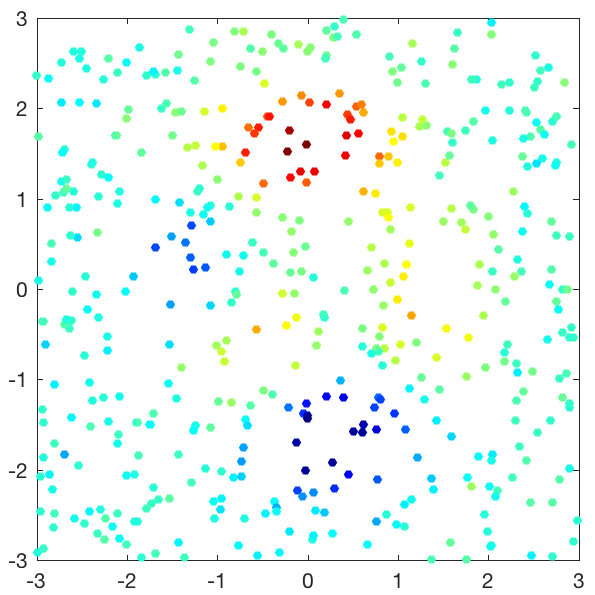
\includegraphics[width=.19\linewidth]{ml/regression/scatter-2d}&
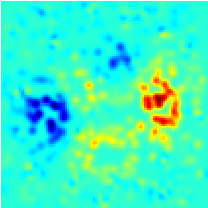
\includegraphics[width=.19\linewidth]{ml/regression/kernel-2}&
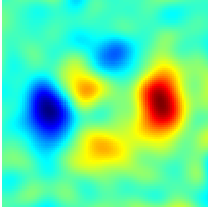
\includegraphics[width=.19\linewidth]{ml/regression/kernel-3}&
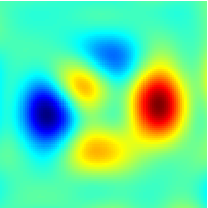
\includegraphics[width=.19\linewidth]{ml/regression/kernel-4}&
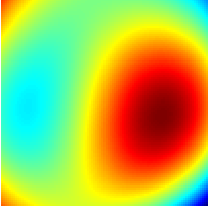
\includegraphics[width=.19\linewidth]{ml/regression/kernel-5}\\
& $\si=0.1$ & $\si=0.5$ & $\si=1$ & $\si=5$
\end{tabular}
\caption{\label{fig-kernel}
Regression using a Gaussian kernel.
}
\end{figure}


The gaussian kernel is the most well known and used kernel
\eq{
	 \kappa(x,y) \eqdef e^{-\frac{\norm{x-y}^2}{2\sigma^2}} . 
}
The bandwidth parameter $\si>0$ is crucial and controls the locality of
the model. It is typically tuned through cross validation.  

Once evaluated on grid points, the kernel define a matrix
\eql{\label{eq-def-kernel-sampled}
	 K = (\kappa(x_i,x_j))_{i,j=1}^n \in \RR^{n \times n}.  
}

Valid kernels are those that gives rise to positive symmetric matrices
$K$. The linear and Gaussian kernel are valid kernel functions. Other
popular kernels include the polynomial kernel $\dotp{x}{y}^a$ for $a
\geq 1$ and the Laplacian kernel $\exp(-\norm{x-y}^2/\si)$.

The weights $\al \in \RR^n $ are solutions of
\eql{\label{eq-min-rkhs}
	 \umin{\al} \norm{K \al-y}^2 + \la_n \dotp{K \al}{\al}  
}
and hence can be computed by solving a linear system
\eq{
	 \al = (K+\la_n \Id_n)^{-1} y  
}
Figure~\eqref{fig-kernel} displays the function $f(\cdot,\al)$ for a varying bandwidth $\si$ for the Gaussian kernel.

This minimization~\eqref{eq-min-rkhs} can be related to an infinite dimensional optimization
problem where one minimizes directly over the function $f$. This
is shown to be equivalent to the above finite-dimenisonal optimization problem
thanks to the theory of RKHS.

%%%%%%%%%%%%%%%%%%%%%%%%%%%%%%%%%%%%%%%%%%%%%%%%%%
%%%%%%%%%%%%%%%%%%%%%%%%%%%%%%%%%%%%%%%%%%%%%%%%%%
%%%%%%%%%%%%%%%%%%%%%%%%%%%%%%%%%%%%%%%%%%%%%%%%%%
\section{Supervised Learning: Classification}
\label{sec-classif}

We now focus on the case of discrete labels $y_i \in \Yy = \{1,\ldots,k\}$, which is the classification setup.
%
We now detail two popular classification methods: logistic and nearest neighbors.
%
It is faire to say that a very large class of successful applications of machine learning technics consists in using one of these two approaches, which should be considered as baselines. 
%
Note that the nearest neighbor approach, while popular for classification could as well be used for regression.

% NN is mostly for low dimensional problems.

 %Logistic for high dimensions.



%%%%%%%%%%%%%%%%%%%%%%%%%%%%%%%%%%%%%%%%%%%%%%%%%%%%%%%%%%%%%%%%%%%%%%%%%%%%%%%%%%%%%%%%%%%%%%%%%%%%%%%%%%%%
\subsection{Nearest Neighbors Classification}


% The opposite of linear regression. 

Probably the simplest method for supervised classification is $R$ nearest neighbors ($R$-NN), where $R$ is a parameter indexing the number of neighbors. Increasing $R$ is important to cope with noise and obtain smoother decision boundary, and hence better generalization performance. It should typically decrease as the number of training sample $n$ increases.

The class $\hat f(x) \in \Yy$ predicted for a point $x$ is the one which is the most represented among the $R$ points $(x_i)_i$ which are the closed to $x$. This is a non-parametric method, and $\hat f$ depends on the numbers $n$ of samples (its ``complexity'' increases with $n$). 

One first compute the Euclidean distance between this $x$ 
and all other $x_{i}$ in the training set. 
%
Sorting the distances generates an indexing $\si$ (a permutation of $\{1,\ldots,n\}$) such that 
\eq{
 	\norm{x-x_{\si(1)}} \leq \norm{x-x_{\si(2)}} \leq \ldots \leq \norm{x-x_{\si(n)}}. 
}
For a given $R$, one can compute the histogram of class apparition
\eq{
 	h_\ell(x) \eqdef \frac{1}{R} \enscond{ i }{ y_{\si(i)} \in \{1,\ldots,R\} }.
}
The decision class for $x$ is then the maximum of the histogram
\eq{
	\hat f(x) \eqdef \uargmax{\ell} h_\ell(x).
}

In practice, the parameter $k$ can be decided through cross-validation, by minimizing the testing risk $R_{\bar n}$ defined in~\eqref{eq-valid-risk}.
%
Of course the method extends to arbitrary metric space in place of Euclidean space $\RR^p$ for the features.
%
Note also that instead of explicitly sorting all the Euclidean distance, one can use fast nearest neighbor search methods.
	
\begin{figure}
\centering
\begin{tabular}{@{}c@{\hspace{3mm}}c@{\hspace{3mm}}c@{\hspace{3mm}}c@{\hspace{3mm}}c@{}}
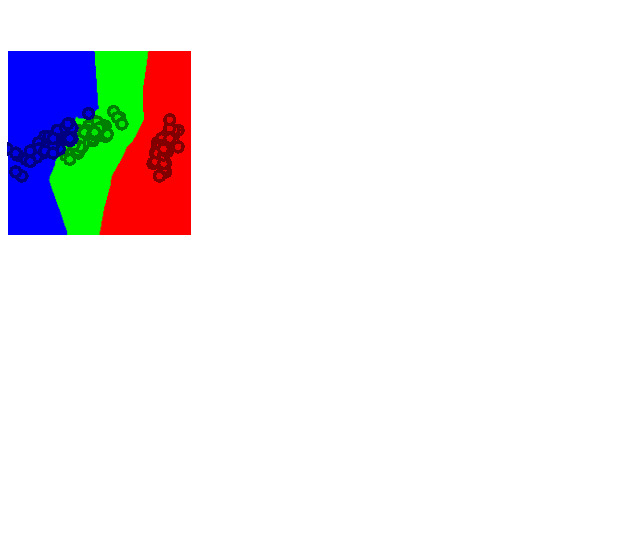
\includegraphics[width=.22\linewidth]{ml/pca-nn/knn-1}&
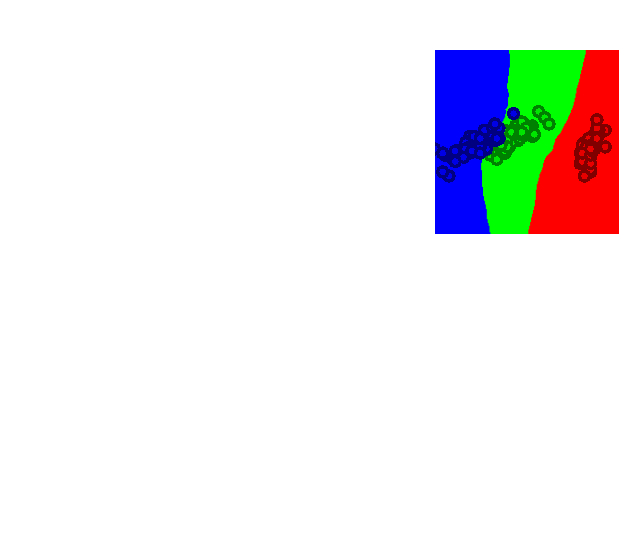
\includegraphics[width=.22\linewidth]{ml/pca-nn/knn-5}&
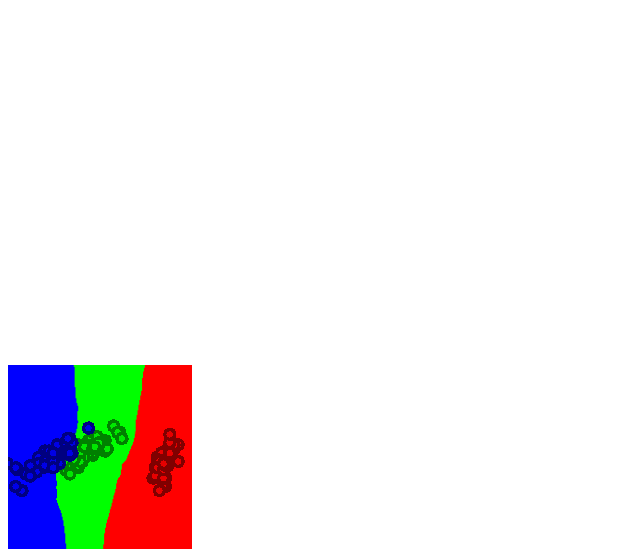
\includegraphics[width=.22\linewidth]{ml/pca-nn/knn-10}&
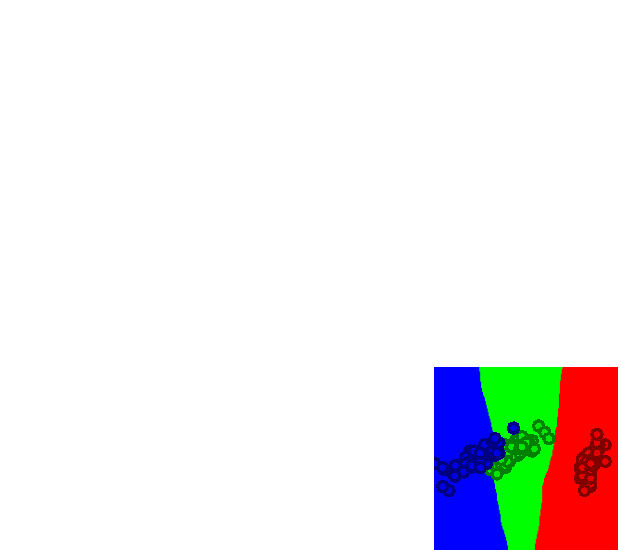
\includegraphics[width=.22\linewidth]{ml/pca-nn/knn-40}\\
$k=1$ & $k=5$ & $k=10$ & $k=40$
\end{tabular}
\caption{\label{fig-hist-classif}
$k$-nearest-neighbor classification boundary function.
}
\end{figure}

Figure~\ref{fig-hist-classif} shows, for the IRIS dataset the classification domain (i.e. $\enscond{x}{f(x)=\ell}$ for $\ell=1,\ldots,k$) in using a 2-D projection for vizualization.
%
Increasing $R$ leads to smoother class boundaries.
%
Despite its simplicity, $k$-NN is surprisingly successful in practice, specially in low dimension $p$.

%%%%%%%%%%%%%%%%%%%%%%%%%%%%%%%%%%%%%%%%%%%%%%%%%%
\subsection{Two Classes Logistic Classification}

The logistic classification method (for 2 classes and
multi-classes) is one of the most popular (maybe ``the'' most) popular machine learning technics. This is due in large part of both its simplicity and because it also output a probability of belonging to each class (in place of just a class membership), which is useful to quantify (somehow \ldots) the ``uncertainty'' of the estimation.
%
Note that logistic classification is actually called ``logistic
regression'' in the literature, but it is in fact a classification method.

Another very popular (and very similar) approach is support vector machine (SVM). SVM is both more difficult to train (because the loss is non-smooth) and does not give class membership probability, so the general rule of thumb is that logistic classification is preferable.

To simplify the expression, classes indexes are set to $y_i \in \Yy = \{-1,1\}$ in the following. Note that for logistic classification, the precision function $f(\cdot,\be) \in [0,1]$ output the probability of belonging to the first class, and not the class indexes. With a slight abuse of notation, we still denote it as $f$. 

Logistic classification can be understood as a linear model as introduced in Section~\ref{sec-linear-models}, although the decision function $f(\cdot,\be)$ is not. Indeed, one needs to ``remap'' the linear value $\dotp{x}{\be}$ in the interval $[0,1]$. In logistic classification, we define the predicted probability of $x$ belonging to class 1 (thus label $-1$) as 
\eq{
	f(x,\be) \eqdef \th(\dotp{x}{\be})
	\qwhereq
   	\th(s) \eqdef \frac{e^{s}}{1+e^s} = (1+e^{-s})^{-1}.
}
Note that the probability of belonging to the second class is $1-f(x,\be)$.

Note that $f(x,\be)$ can be interpreted as a single layer perceptron with a logistic (sigmoid) rectifying unit. 

Since the $(x_i,y_i)$ are modelled as i.i.d. variables, it makes sense to define $\hat \be$ from the observation using a maximum likelihood, assuming that each $y_i$ conditionned on $x_i$ is a Bernoulli variable with associated probability $(p_i,1-p_i)$ with $p_i=f(x_i,\be)$. The probability of oberving $y_i \in \{0,1\}$ is thus, denoting $s_i=\dotp{x_i}{\be}$
\eq{
	\PP(\yp=y_i|\xp=x_i) =p_i^{\bar y_i} (1-p_i)^{1-\bar y_i}
	= \pa{
		\frac{e^{s_i}}{1+e^{s_i}}
	}^{1-\bar y_i} 
	\pa{
		\frac{1}{1+e^{s_i}}
	}^{\bar y_i}
}
where we denoted $\bar y_i = \frac{y_i+1}{2} \in \{0,1\}$.

One can then minimize minus the sum of the log of the likelihoods, which reads
\eq{
	\hat\be \in \uargmin{\be \in \RR^p} 
		- \sum_{i=1}^n \log( \PP(\yp=y_i|\xp=x_i) ) = 
		\sum_{i=1}^n - (1-\bar y_i) \log \frac{e^{s_i}}{1+e^{s_i}}
			- \bar y_i\log \frac{1}{1+e^{s_i}}
}
Some algebraic manipulations shows that this equivalent to an ERM-type form~\eqref{eq-erm-1} with a logistic loss function 
\eql{\label{eq-logistic-optim}
	\hat\be \in \uargmin{\be \in \RR^p} 
		 E(\be)  = \frac{1}{n} \sum_{i=1}^n \Ll(\dotp{x_i}{\be},y_i)  
}
where the logistic loss reads
\eq{
	 \Ll( s,y ) \eqdef \log( 1+\exp(-sy) ). 
}
Problem~\eqref{eq-logistic-optim} is a smooth convex minimization. If $X$ is injective, $E$ is also strictly convex, hence it has a single global minimum.

\begin{figure}
\centering
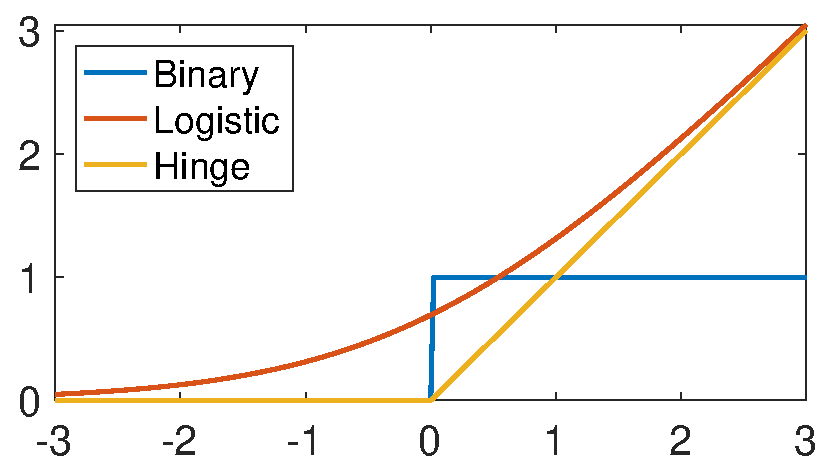
\includegraphics[width=.4\linewidth]{ml/classif/losses}
\caption{\label{fig-losses}
Comparison of loss functions. 
}
\end{figure}

Figure~\eqref{fig-losses} compares the binary (ideal) 0-1 loss, the logistic loss and the hinge loss (the one used for SVM).

Re-writting the energy to minimize
\eq{
	 E(\be) = \tilde\Ll(X \be,y) \qwhereq \tilde\Ll(s,y)= \frac{1}{n}  \sum_i \Ll(s_i,y_i), 
}
its gradient reads
\eq{
	 \nabla E(\be) = X^\top \nabla \tilde\Ll(X \be,y)
      \qwhereq
      \nabla \tilde\Ll(s,y) = \frac{y}{n} \odot \th(-y \odot s),   
}
where $\odot$ is the pointwise multiplication operator, i.e. \texttt{.*} in Matlab.
%
Once $\be^{(\ell=0)} \in \RR^{p}$ is initialized (for instance at $0_{p}$), one step of gradient descent~\eqref{eq-grad-desc} reads
\eq{
	 \iit{\be} = \it{\be} - \tau_\ell \nabla E(\it{\be}). 
}

% In order to improve performance, it is important (especially in low dimension $p$) to add a constant bias term $\be_{p+1} \in \RR$, and replace $\dotp{x_i}{\be}$ by $ \dotp{x_i}{\be} + \be_{p+1} $.  This is equivalently achieved by adding an extra $(p+1)^{\text{th}}$ dimension equal to 1 to each $x_i$, which we do using a convenient macro.




\begin{figure}
\centering
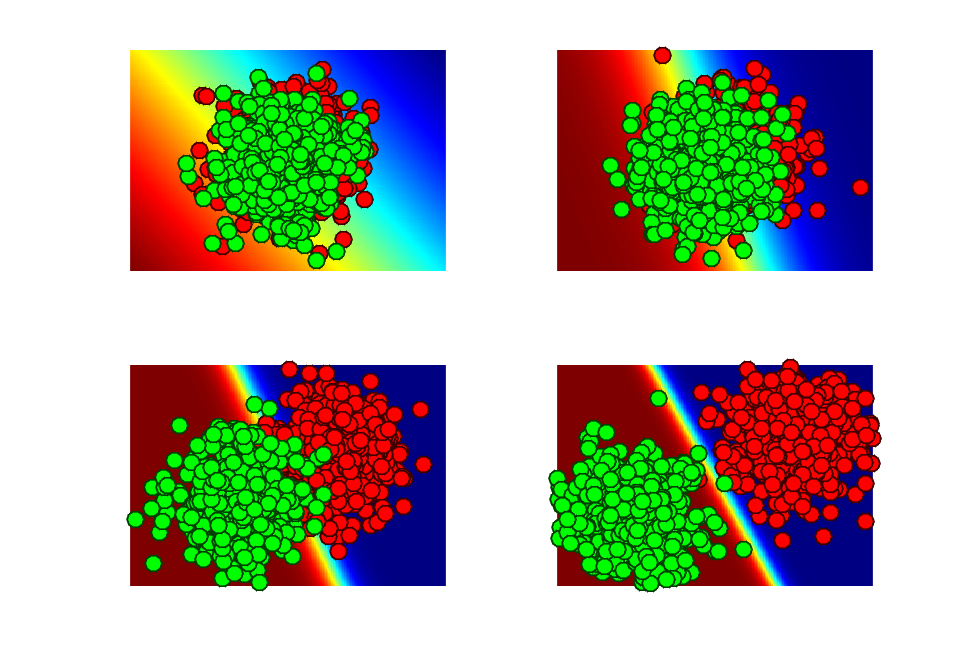
\includegraphics[width=.4\linewidth]{ml/classif/classes-2-separation-influ}
\caption{\label{fig-separation-influ}
Influence on the separation distance between the class on the classification probability. 
}
\end{figure}

To understand the behavior of the method, in Figure~\ref{fig-separation-influ} we generate synthetic data distributed according to a mixture of Gaussian with an overlap governed by an offset $\omega$. 
%
One can display the data overlaid on top of the classification probability, this highlight the separating hyperplane $\enscond{x}{\dotp{\be}{x}=0}$.



%%%%%%%%%%%%%%%%%%%%%%%%%%%%%%%%%%%%%%%%%%%%%%%%%%%%%%%%%%%%%%%%%%%%%%%%%%%%%
\subsection{Kernelized Logistic Classification}

Logistic classification tries to separate the classes using
a linear separating hyperplane $ \enscond{x}{\dotp{w}{x}=0}$. 

In order to generate a non-linear decision boundary, one can replace the
parametric linear model by a non-linear non-parametric model, thanks to
kernelization. It is non-parametric in the sense that the number of
parameter grows with the number $n$ of sample (while for the basic
method, the number of parameter is $p$). This allows in particular to
generate decision boundaries of arbitrary complexity.

The downside is that the numerical complexity of the method grows
(at least) quadratically with $n$.

The good news however is that thanks to the theory of reproducing kernel Hilbert spaces
(RKHS), one can still compute this non-linear decision
function using (almost) the same numerical algorithm.

Similarly to~\eqref{eq-kernelized-function}, given a kernel $\kappa(x,z) \in \RR$ defined for $(x,z) \in \RR^p$,
the kernelized method replace the linear decision functional $f(x) =
\dotp{x}{\be}$ by a sum of $f(x,\al)$ of kernel centered on the samples
\eq{
	 f(x,\al) = \sum_{i=1}^n \al_i k(x_i,x) 
}
where $\al \in \RR^n$ is the unknown vector of weight to find.

\begin{figure}
\centering
\begin{tabular}{@{}c@{\hspace{5mm}}c@{}}
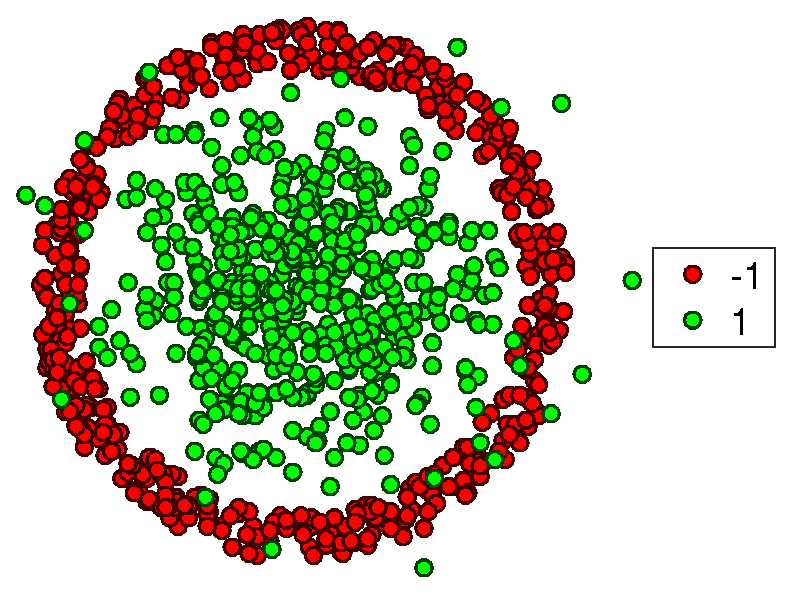
\includegraphics[width=.35\linewidth]{ml/classif/classes-kernel}&
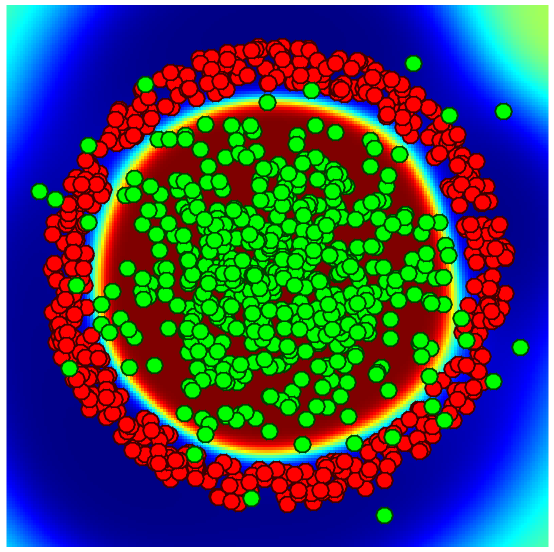
\includegraphics[width=.25\linewidth]{ml/classif/classes-kernel-result}
\end{tabular}
\caption{\label{fig-classes-kernel}
Non-linear classification using a Gaussian kernel.
}
\end{figure}


The kernelized Logistic minimization reads
\eq{
	 \umin{\al \in \RR^n} F\Ff(\al) \eqdef \tilde\Ll(K \al,y)
}
where $K$ is the sampled kernel~\eqref{eq-def-kernel-sampled}.
%
One can then use a gradient descent to minimize $\Ff(\al)$.

Once this optimal $\al$ has been found, class probability at a point
$x$ are obtained as
\eq{
	 (\th(f(x,\al)), 1-\th(f(x,\al)) 
}
where $f(\cdot,\al)$ is defined in~\eqref{eq-kernelized-function}.

Note that it is of course possible to add a regularization to this problem
\eq{
	 \umin{\al} \tilde\Ll(K \al,y) + \la R(\al), 
}
where for instance $R=\norm{\cdot}_2^2$ or $R=\norm{\cdot}_1$.


%%%%%%%%%%%%%%%%%%%%%%%%%%%%%%%%%%%%%%%%%%%%%%%%%%%%%%%%%%%%
\subsection{Multi-Classes Logistic Classification}

The logistic classification method is extended to an arbitrary number
$k$ of classes by considering a family of weight vectors $\be = ( \be_\ell )_{\ell=1}^k $, which are conveniently stored as columns of matrix $\be \in \RR^{p \times k}$.

This allows one to model probabilistically the belonging of a point $x \in \RR^p$ to 
the classes using an exponential model
\eq{
	 h(x) = \pa{ \frac{ e^{-\dotp{x}{\be_\ell}} }{ \sum_m e^{-\dotp{x}{\be_m}} } }_\ell 
}
This vector $h(x) \in [0,1]^k$ describes the probability of $x$
belonging to the different classes, and $\sum_\ell h(x)_\ell = 1$.

The computation of $\be$ is obtained by solving a maximum likelihood
estimator
 \eq{
	 \umax{\be \in \RR^{p \times k}} \frac{1}{n} \sum_{i=1}^n \log( h(x_i)_{y_i} ) 
}
where we recall that $y_i \in \Yy = \{1,\ldots,k\}$ is the class index of
the point $x_i$.

This is conveniently rewritten as
\eq{
	 \umin{\be \in \RR^{p \times k}} \Ee(\be) \eqdef \sum_i \text{LSE}( X \be )_i - \dotp{X \be}{D} 
}
where $D \in \{0,1\}^{n \times k}$ is the binary class index matrices
\eq{
	  D_{i,\ell} = \choice{
          1 \qifq y_i=\ell, \\
          0 \text{otherwise}.
      }
}
and LSE is the log-sum-exp operator
\eq{
	 \text{LSE}(S) = \log\pa{ \sum_\ell \exp(S_{i,\ell}) } \in \RR^n. 
}


The computation of LSE is
unstable for large value of $S_{i,\ell}$ (numerical overflow, producing NaN), but this can be
fixed by subtracting the largest element in each row,
since $ \text{LSE}(S+a)=\text{LSE}(S)+a $ if $a$ is constant along rows. This is often referred to as 
the ``LSE trick''.





The gradient of the LSE operator is the soft-max operator
\eq{
	  \nabla \text{LSE}(S) = \text{SM}(S) \eqdef
      \pa{
          \frac{
                  e^{S_{i,\ell}}
              }{
                  \sum_m e^{S_{i,m}}
              } }   
}
Similarly to the LSE, it needs to be stabilized.


\begin{figure}
\centering
\begin{tabular}{@{}c@{\hspace{5mm}}c@{\hspace{5mm}}c@{}}
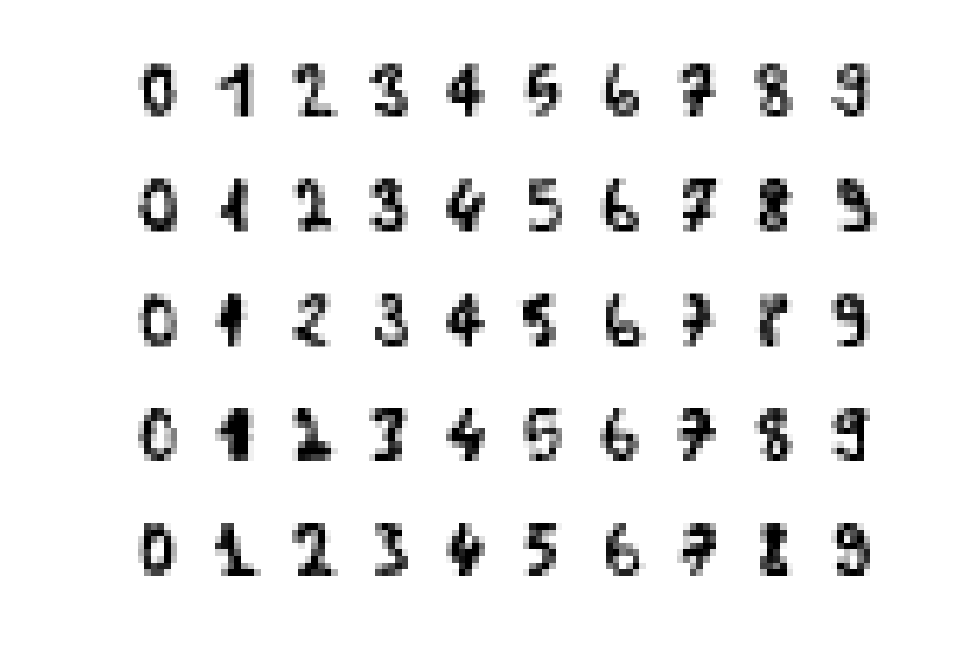
\includegraphics[width=.25\linewidth]{ml/classif/digits}&
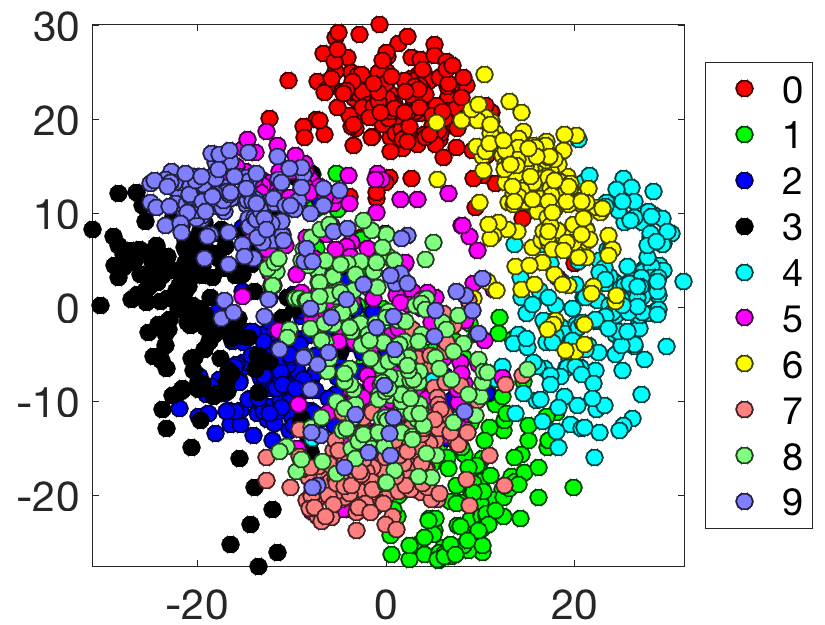
\includegraphics[width=.25\linewidth]{ml/classif/digits-2d}&
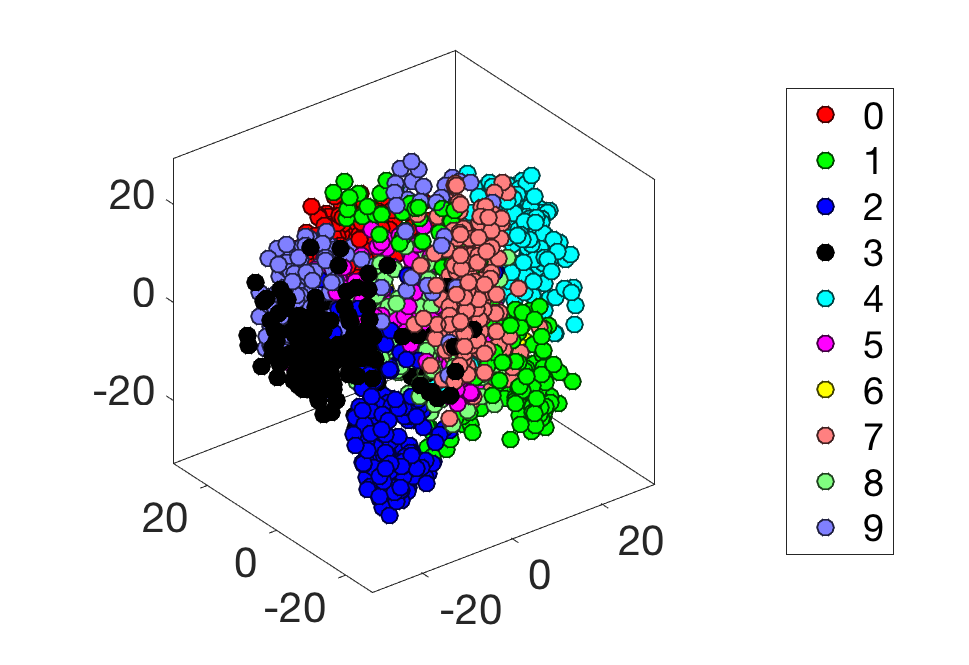
\includegraphics[width=.25\linewidth]{ml/classif/digits-3d}
\end{tabular}
\caption{\label{fig-digits}
2-D and 3-D PCA vizualization of the digits images.
}
\end{figure}

We load a dataset of $n$ images of size $p = 8 \times 8$, representing digits from 0
to 9 (so there are $k=10$ classes).
%
Figure~\ref{fig-digits} displays a few representative examples as well as 2-D and 3-D PCA projections.



Once $D$ matrix is computed, the gradient of $\Ee$ is computed as 
\eq{
	 \nabla \Ee(\be) =  \frac{1}{n} X^\top ( \text{SM}(X \be) - D ).  
}
and one can minimize $\Ee$�using for instance a gradient descent scheme.
%
Figure~\eqref{fig-digits-classes} displays the ``fuzzy'' decision boundary by vizualizing the value of $h(x)$ using colors on an image regular grid.

\begin{figure}
\centering
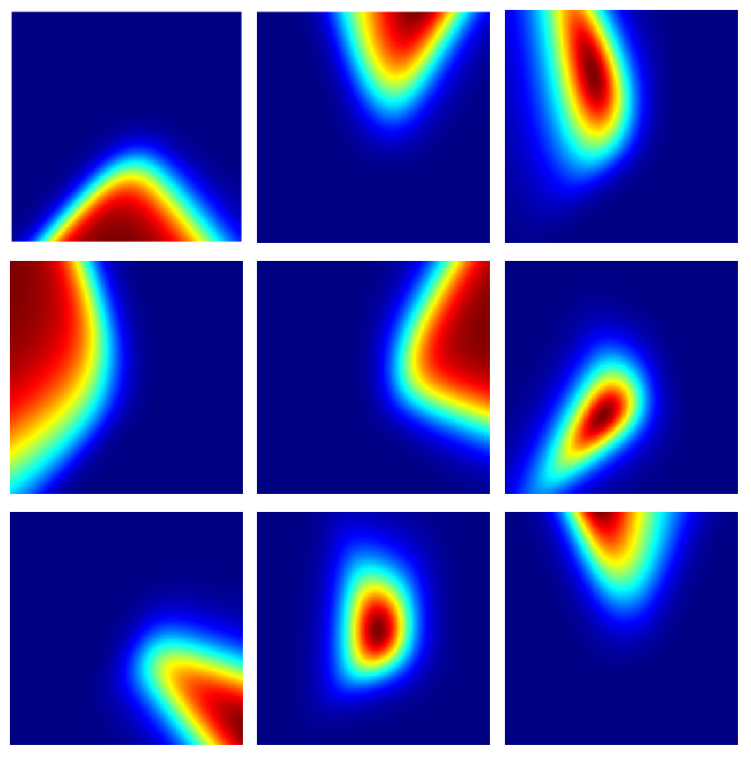
\includegraphics[width=.35\linewidth]{ml/classif/digits-classes}
\qquad
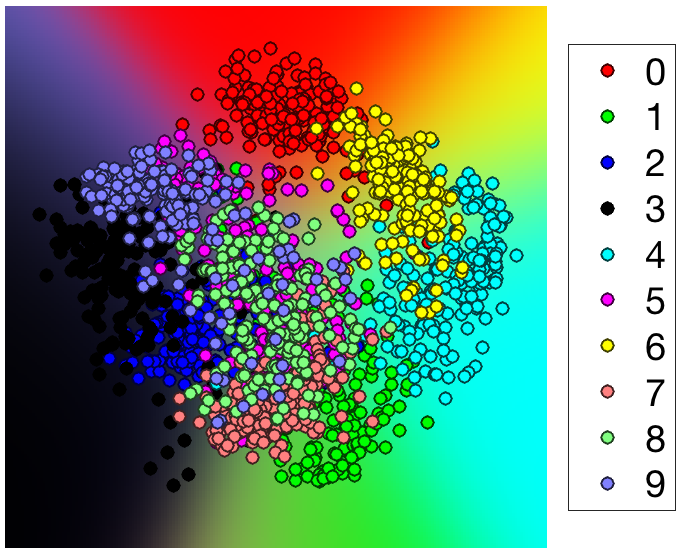
\includegraphics[width=.44\linewidth]{ml/classif/digits-classes-single}
\caption{\label{fig-digits-classes}
Results of digit classification
Left: probability of belonging to each of the 9 first classes (displayed over a 2-D PCA space).
Right: colors reflect probability of belonging to classes.
}
\end{figure}


